\begin{figure}[th]
\centering
\subfigure[C$\rightarrow$A]{
    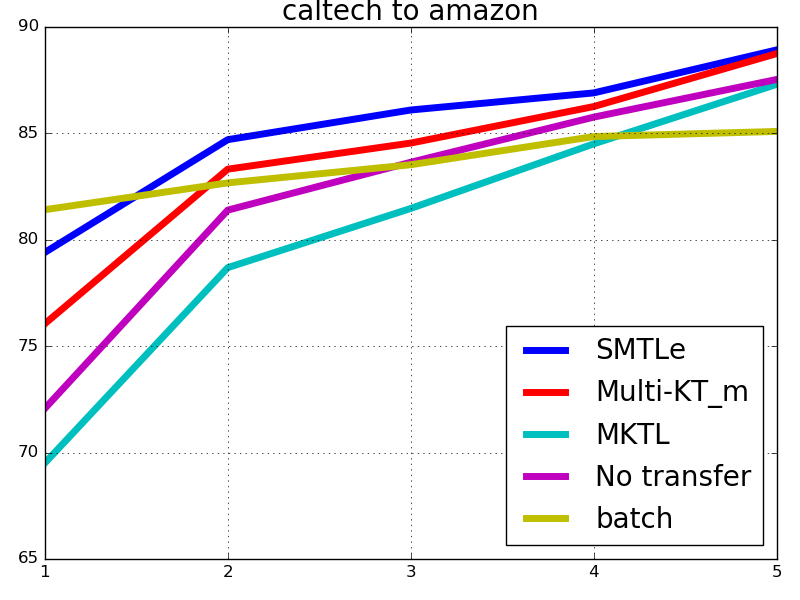
\includegraphics[width=0.22\textwidth]{fig/caltechtoamazon.png}\label{a}
}
\subfigure[D$\rightarrow$A]{
    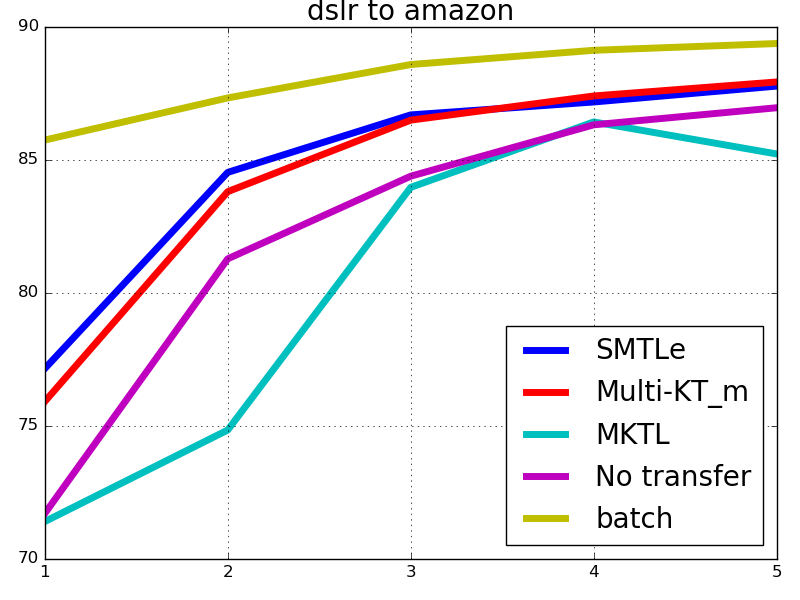
\includegraphics[width=0.22\textwidth]{fig/dslrtoamazon.png}\label{b}
}
\subfigure[W$\rightarrow$A]{
	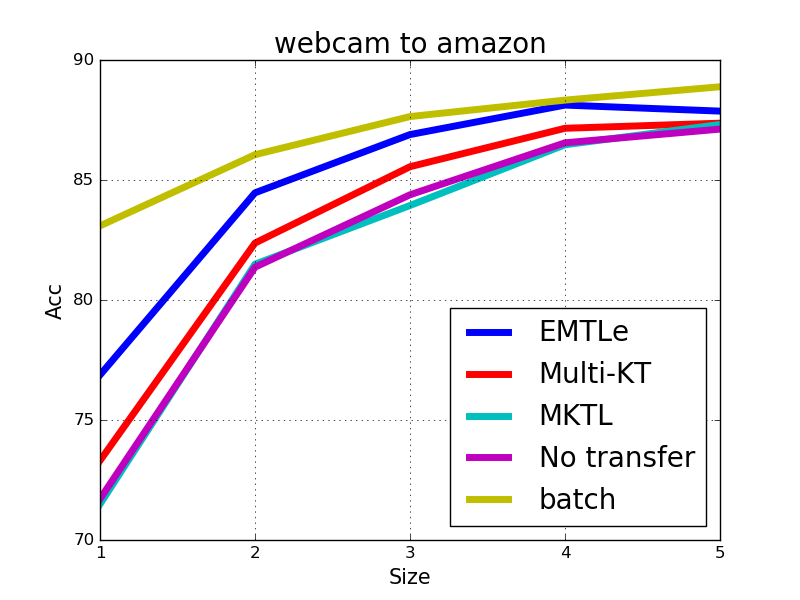
\includegraphics[width=0.22\textwidth]{fig/webcamtoamazon.png}\label{c}
}
\subfigure[A$\rightarrow$C]{
	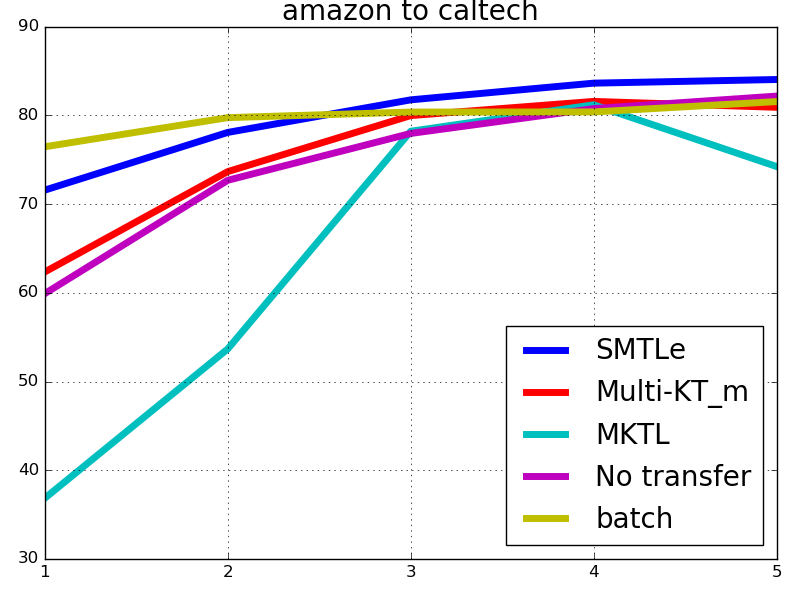
\includegraphics[width=0.22\textwidth]{fig/amazontocaltech.png}\label{d}
}\\
\subfigure[D$\rightarrow$C]{
	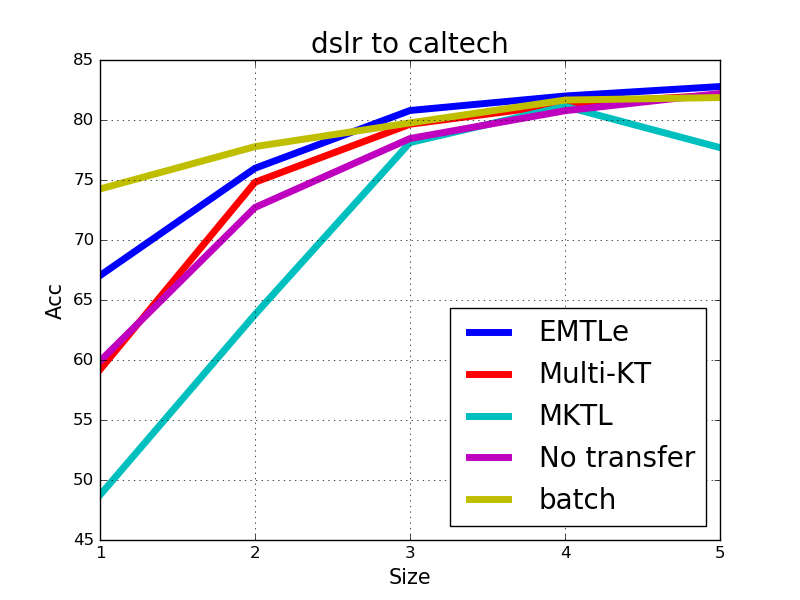
\includegraphics[width=0.22\textwidth]{fig/dslrtocaltech.png}\label{e}
}
\subfigure[W$\rightarrow$C]{
	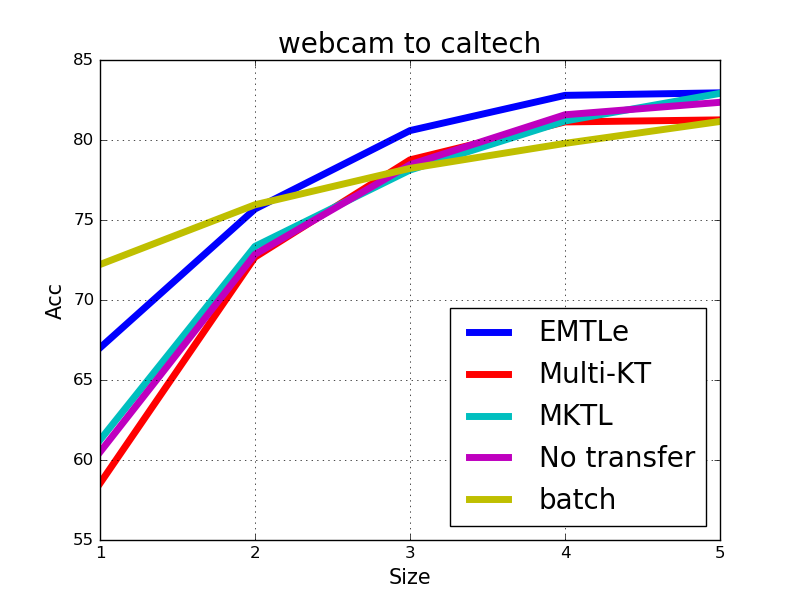
\includegraphics[width=0.22\textwidth]{fig/webcamtocaltech.png}\label{f}
}
\subfigure[A$\rightarrow$D]{
	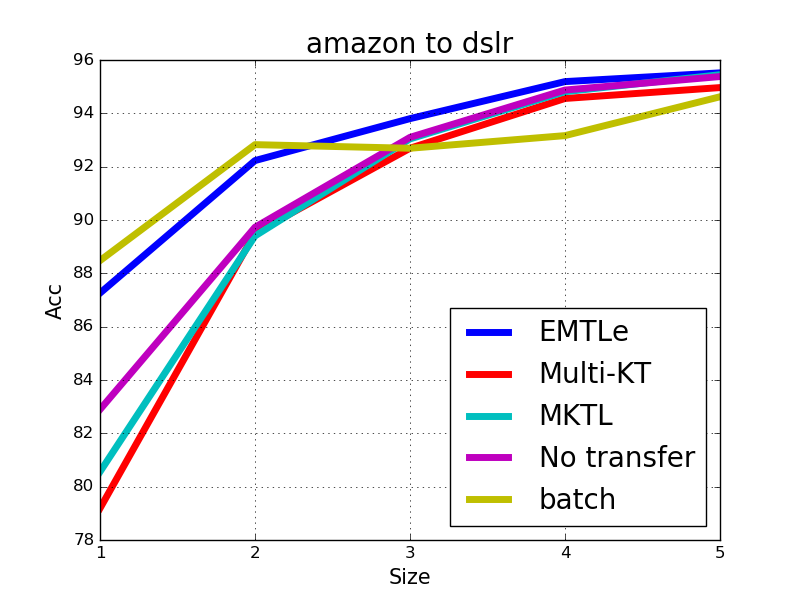
\includegraphics[width=0.22\textwidth]{fig/amazontodslr.png}\label{g}
}
\subfigure[C$\rightarrow$D]{
	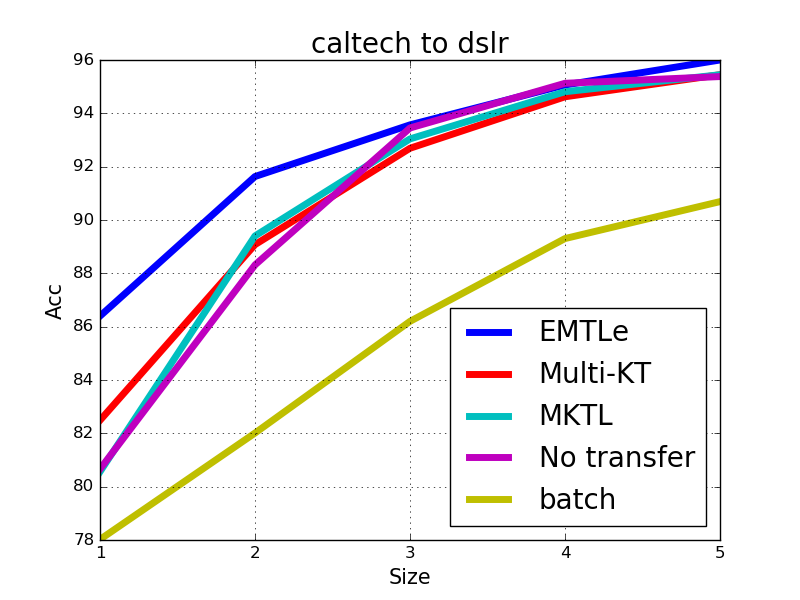
\includegraphics[width=0.22\textwidth]{fig/caltechtodslr.png}\label{h}
}\\
\subfigure[W$\rightarrow$D]{
	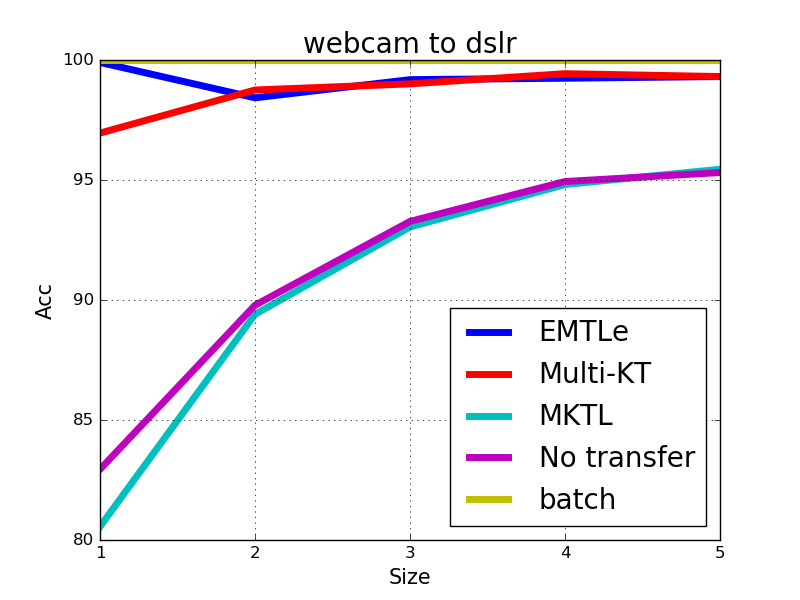
\includegraphics[width=0.22\textwidth]{fig/webcamtodslr.png}\label{i}
}
\subfigure[A$\rightarrow$W]{
	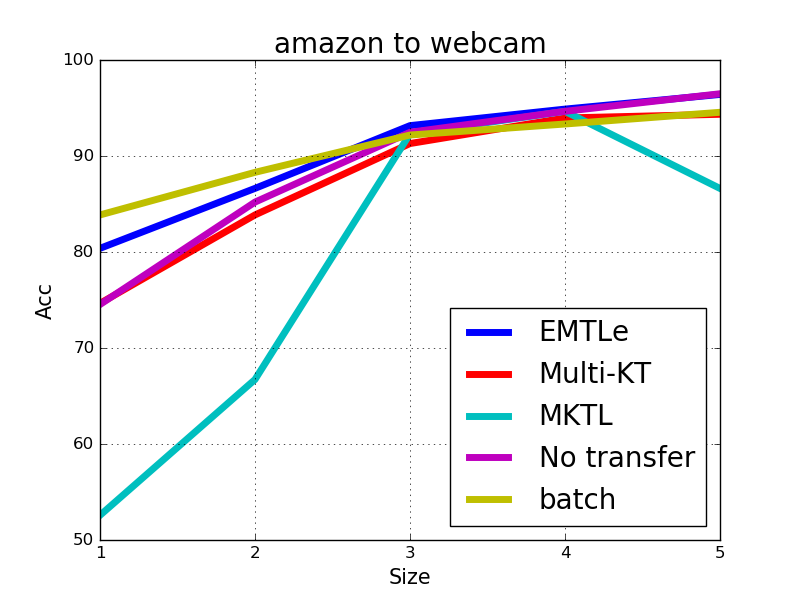
\includegraphics[width=0.22\textwidth]{fig/amazontowebcam.png}\label{j}
}
\subfigure[C$\rightarrow$W]{
	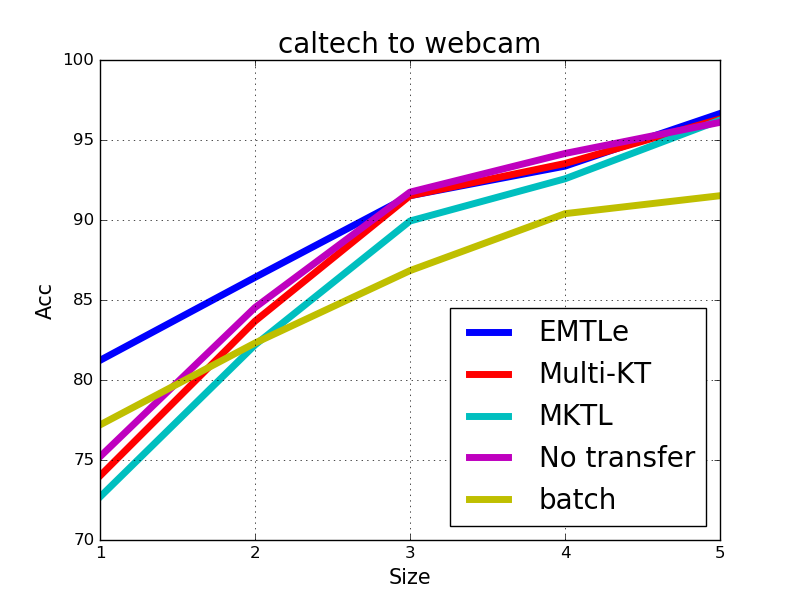
\includegraphics[width=0.22\textwidth]{fig/caltechtowebcam.png}\label{k}
}
\subfigure[D$\rightarrow$W]{
	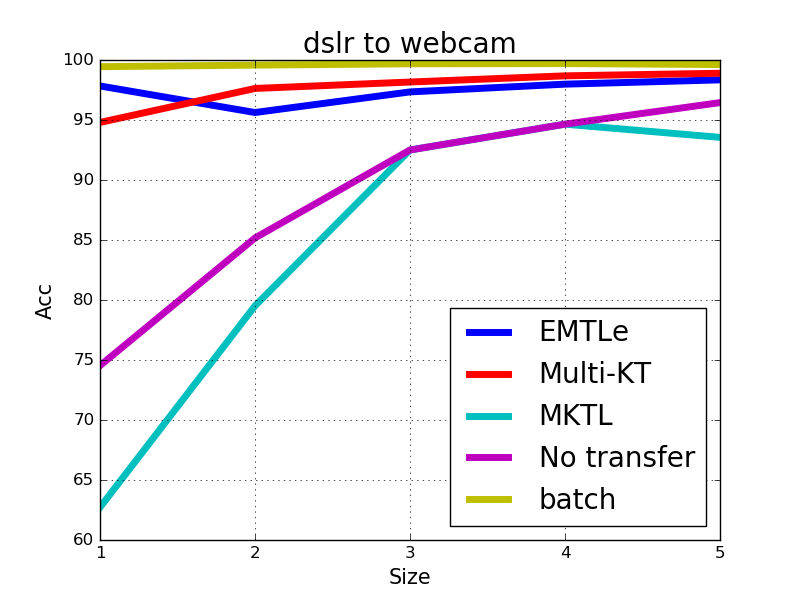
\includegraphics[width=0.22\textwidth]{fig/dslrtowebcam.png}\label{l}
}
\caption{Recognition accuracy for HTL domain adaptation using single source single source classifier. 5 different sizes of target training sets are used in each group of experiments.}
\label{fig:exp}
\end{figure}

\textbf{Observation \& discussion:} EMTLe can significantly outperform other baselines especially when the training size is small. %Moreover, in some groups of experiments, they even suffer from negative transfer on the small training set. 
As we have discussed above, when the training set is small, with the transfer parameter estimated by our $\ell_2$ penalty in our high-level objective functions, EMTLe has a strong generalization ability and performs better on the test data. As the training size increases, the variance of training data decreases and the affect of the $\ell_2$ penalty term become less significant. Therefore, EMTLe and the other two HTL baselines show similar performance. 
It is interesting to see that MKTL even fall into negative transfer even with 5 training examples per class in some experiments. We found that, MKTL is more sensitive to variance of the training data its performance is not as stable as Multi-KT and EMTLe over the 10 rounds experiments. Because MKTL need to learn more hyperparameters than Multi-KT and EMTLe, even though the training size increases, it may not be able to obtain a good model. 
In some experiments, we can see that EMTLe can even outperform the Batch method which which can access more information and is expected to outperform the other methods under the setting of HTL.